\section{Licht und Farbe}
\authors{Ailin Sigel, Selin Güler}

Um zu verstehen, wie Farbigkeit zustande kommt, sollte man zunächst erwähnen, dass Licht einen Wellencharakter und spezifische Welleneigenschaften hat. Die Lichtwellen lassen sich nach ihrer Länge und  enthaltenden Energie im Spektrum elektromagnetischer Wellen einordnen.

Menschen können nur einen kleinen Teil des elektromagnetischen Spektrums wahrnehmen, den so genannten sichtbaren Bereich (siehe Abbildung \ref{dsafigure:beispiel}). Dieser erstreckt sich über Wellenlängen von 380 nm bis 780 nm und beinhaltet die Farben Violett, Blau, Grün, Gelb, Orange und Rot. 

\begin{dsafigure}
 \centering
 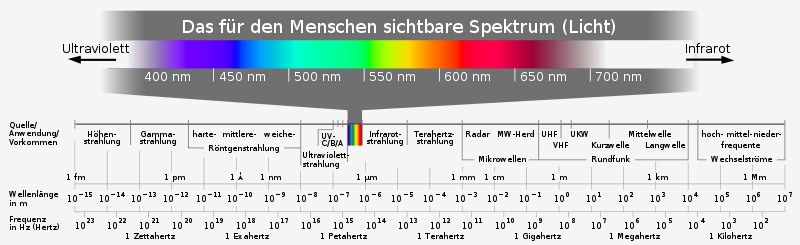
\includegraphics[width=\columnwidth]{pics/elektromagnetisches_Spektrum.png}
 \caption{Elektromagnetisches Spektrum mit dem für den Menschen sichtbaren Bereich des Spektrums.  \cite{elektromagnetisches_Spektrum}}
 \label{dsafigure:beispiel}
\end{dsafigure}

Das Sonnenlicht enthält alle Farben dieses Farbspektrums und erscheint deshalb weiß. Wenn die Lichtquelle ausgeschaltet ist, sehen wir schwarz, da kein Licht ausgestrahlt wird. Wird bei diesem additiven Farbsystem zum Beispiel das Licht von einer blauen und einer roten Lampe addiert, entsteht die Farbe Magenta (siehe Abbildung \ref{dsafigure:farbkreis}). Im Gegensatz dazu wird das Licht einer Lichtquelle (zum Beispiel der Sonne) von allen Gegenständen reflektiert. 
Bei diesem substraktivem Farbsystem ergibt sich die Farbe Schwarz aus der gemeinsamen Absorption von Wellenlängen aller Farben (siehe Abbildung \ref{dsafigure:farbkreis}).

Den Zusammenhang zwischen der Wellenlänge und der Energie lässt sich mit folgender Formel erklären:

\begin{equation}
E = \frac{h \cdot c}{\lambda} 
= h \cdot \nu
\end{equation}

$E$ beschreibt die Energie des Photons, $h$ das Plancksches Wirkungsquantum, $c$ die Lichtgeschwindigkeit, $\lambda$ die Wellenlänge, und $\nu$ die Frequenz.
Bei einer höheren Energie hat das Licht eine höhere Frequenz und dementsprechend ist die Wellenlänge kürzer. Umgekehrt bedeutet es auch, dass das Licht bei einer niedrigeren Energie eine niedrigere Frequenz und somit auch eine längere Wellenlänge hat.

\begin{dsafigure}
 \centering
 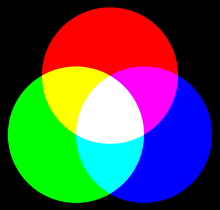
\includegraphics[width=0.45\columnwidth]{Additives_Farbsystem.png}
  \hfill
 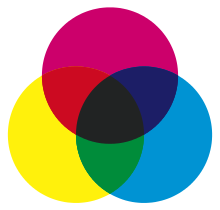
\includegraphics[width=0.45\columnwidth]{Substraktives_Farbsystem.png}
 \caption{Additives Farbsystem (links)\cite{Additives_Farbsystem} und Substraktives Farbsystem (rechts)\cite{Subtraktives_Farbsystem}}
 \label{dsafigure:farbkreis}
\end{dsafigure}


Der Zusammenhang zwischen Licht und Farbigkeit liegt an der Absorption und Reflexion von Licht. Dieses fällt durch die Pupille ins Auge und trifft dort auf die Netzhaut, die wiederum aus Stäbchen und Zapfen besteht. Die Stäbchen sind bei schwachen Lichteinfall aktiv und wir können damit nur schwarz-weiß sehen. Die Zapfen befinden sich im Zentrum der Netzhaut und sind besonders bei hohem Lichteinfall aktiv. Es gibt drei unterschiedliche Arten von Zapfen, die s-Zapfen, die als blaue Rezeptoren fungieren, die m-Zapfen, die als grüne Rezeptoren fungieren und die l-Zapfen, die als rote Rezeptoren fungieren. Jeder der Zapfen hat sein Maximum bei einer anderen Wellenlänge und zusammen decken sie somit den sichtbaren Bereich des elektromagnetischen Spektrums ab. 
Bei Anregung der Zapfen durch Licht, leiten sie einen Reiz an das Gehirn weiter. Durch die Kombination der verschiedenen angeregten Zapfen sehen wir Farbe.
Betrachten wir einen blauen Stift, der von der Sonne angeleuchtet wird, dann erscheint er uns blau. Was wir allerdings nicht sehen ist, dass die Elektronen im Stift vom Licht angeregt werden und vom Grundzustand in ein höheres Energieniveau angehoben werden (siehe Abbildung \ref{dsafigure:Grundzustand} ). Da dieser Zustand sehr instabil ist, fällt das Elektron wieder in seinen Grundzustand zurück. Dabei erfolgt die so genannten Relaxation über Schwingungen des Systems und es entsteht Wärme (siehe Abbildung \ref{dsafigure:Grundzustand}). Dass wir den Stift als blau wahrnehmen liegt daran, dass er die Komplementärfarbe zu Blau, also Gelb, absorbiert. Durch das fehlen der gelben Wellenlänge im reflektiertem Licht des Stiftes, interpretiert das Gehirn ihn als blau (siehe Abbildung \ref{dsafigure:farbkreis}, additives Farbsystem).
Wird blaues Licht durch einen Prozess emittiert, wird dieses ebenfalls als blau wahrgenommen.


\begin{dsafigure}
 \centering
 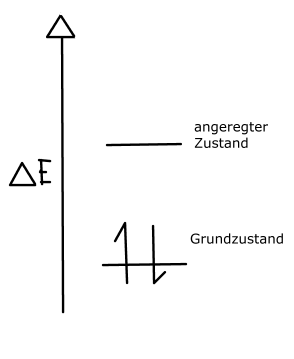
\includegraphics[width=0.45\columnwidth]{Grundzustand.png}
   \hfill
   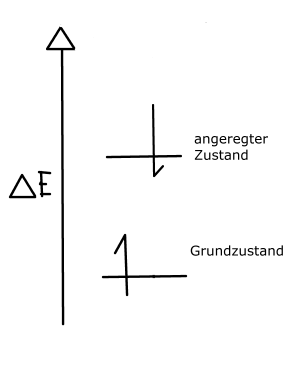
\includegraphics[width=0.45\columnwidth]{angeregter_Zustand.png}
 \caption{Elektronen im Grundzustand (links) und im angeregten Zustand (rechts)}
 \label{dsafigure:Grundzustand}
\end{dsafigure}

